%
% Template file for software architecture design description in the
% DIKU course Software Architecture and Software Design. Please do
% not distribute outside the course
%
% Based on a template (c) by Woods and Rozanski (2011) available at
%
%    http://www.viewpoints-and-perspectives.info
%
% Instructions:
%
% 1) change the metadata commands below (\groupname) etc. to fit your
%     project
% 2) uncomment the overwriting of the \instructions command to remove
%     instructions
% 3) write your architectural description...
%
% Contact: klausmh@di.ku.dk
%
\documentclass[a4paper,11pt]{report}
\usepackage{natbib}
\usepackage[pdftex]{graphicx}
\usepackage{color}
\usepackage[table]{xcolor}
\usepackage{hyperref}
\usepackage{lastpage}

% Meta-data for report
\newcommand{\systemname}{Online Rental System}
\newcommand{\groupname}{Group $\Omega$}
\newcommand{\contactdetails}{Henrik Bendt: gwk553@ku.dk\\Nicolai Willems ntb459@ku.dk\\Søren Egede Pilgård: vpb984@ku.dk}

% Typesetting of instructions for using the template,
% remove by renewing command
\newcommand{\instructions}[1]{
  \noindent\colorbox{lightgray}{%
    \parbox{\linewidth}{%
      #1
    }%
  }%
 \vspace{0.1cm}
}
\renewcommand{\instructions}[1]{} % Uncomment to remove instructions

% We use the below command for figure captions since
% the figure environment does not play nicely with
% \colorbox. The "real" way to create figures is like this:
%   \begin{figure}[ht!]
%     \centering
%     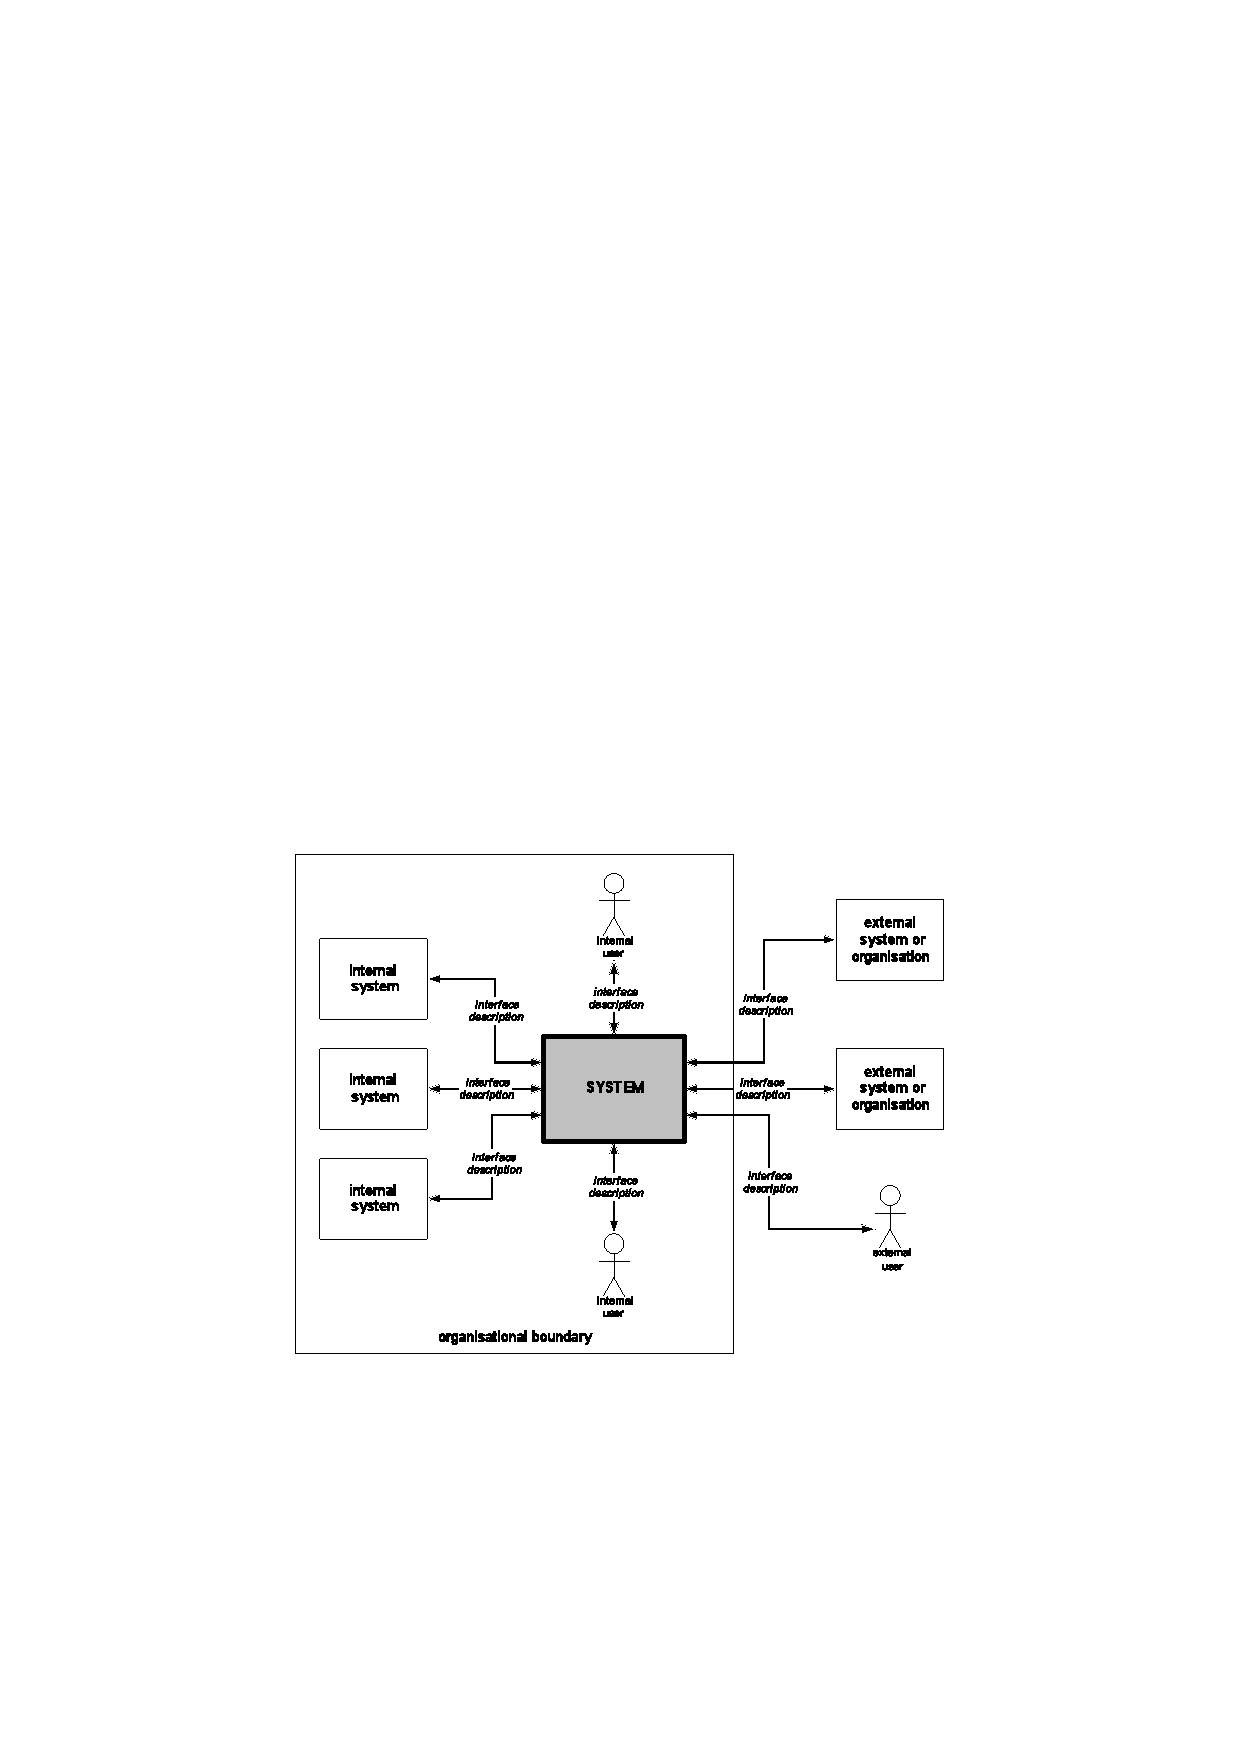
\includegraphics[width=0.8\textwidth]{figures/systemcontext}
%    \caption{System context}
%     \label{fig:systemcontext}
%   \end{figure}
\newcommand{\mycaption}[1]{
  \addtocounter{figures}{1}
  Figure \arabic{figures}. #1
}

\setlength\parskip{1em}
\setlength\parindent{0em}

% Change font family to Helvetica
\renewcommand{\rmdefault}{phv}
\renewcommand{\sfdefault}{phv}

% Set headers and footers
\usepackage{fancyhdr}
\pagestyle{fancy}
\fancyhf{}
\fancyhead[C]{Software Architecture of \systemname\ }
\fancyfoot[C]{\footnotesize Page \thepage\ of \pageref{LastPage}}


\begin{document}
%
% Title page
%
\newcommand{\HRule}{\rule{\linewidth}{0.5mm}}
\begin{titlepage}

  \begin{center}

    % Title
    \vspace*{4cm}
    \HRule \\[0.4cm]
    { \huge \bfseries \systemname}\\[0.4cm]
    \HRule \\[1.5cm]

    {\Large Software Architecture Description}

    \vfill
  \end{center}

  % Author, version, date
  \begin{flushleft}
    {\LARGE \groupname}\\[0.2cm]
    {\large \contactdetails}\\[0.2cm]
   {\large \today}
  \end{flushleft}
\end{titlepage}

%
% Version table
%
\newpage
\chapter*{Version history}

\begin{center}
  \begin{tabular}[h!]{| l | l | l | p{8 cm} |}
    \hline
    \rowcolor{gray}
    Version & Date & Author & Comments \\
    \hline
    \hline
    1 & 2014-09-03 & HB & Filling out ch 1 and 5.1\\
    \hline
    2 & 2014-09-08 & NW & Adding figure and group name \\
  \end{tabular}
\end{center}

%
% Table of contents
%
\setcounter{tocdepth}{1}
\tableofcontents

%
% Main text
%
\chapter{Introduction}
\label{cha:introduction}
\thispagestyle{fancy}


\section{Purpose and scope}
\label{sec:purpose-scope}
The project is about developing an online renting system (as a website), from
here on referred to as ORS. In the system it should be possible for users to
rent out items to other users for a small fee (possibly none) and a safety
deposit (in case of return of damaged items). When a user wants to rent a
provided item, the system should provide the contact information to the
providing user. The business case is to take a small percentage or amount from
the rental fee when providing the contact information.

Users should be able to search for specific items or item categories,
geographical locations, price ranges, etc. They should also be able to queue up
for a specific provided item (by another user) if it is already rented out or
multiple other people are interested in renting the item.

It should be possible to share what you are renting out on Facebook or Twitter.

A scenario could be a person, owning an electric saw, which he is not using, but
don't want to sell. He could then be interested in making some money off this
item, by renting it to people in his area (for example his home city Copenhagen,
or maybe in all of Sjælland, etc.). Instead of setting up fliers in his local
area (like in the local grocery store, local sports center, etc.) he puts the
item up on ORS because it is easy and fast. Now, people in need of such electric
saw contacts him without him doing anything but making the electric saw
available for renters.

The system is to be deployed and runned on a cloud system like Amazon Cloud. It should use an external paying system like Paypal.

\subsection{Scope}
\paragraph{Included}
\begin{itemize}
\item Supplie items for rent
\item Search for items for rent
\item Requests items for rent
\item Billing + Deposits when renting
\item Tracking of items rented out (which user, living where)
\item Website handling the above
\end{itemize}

\paragraph{Excluded}
\begin{itemize}
\item Sales
\item Errors + Damage to items -- handling these cases
\item Hardware for the server -- we shall use a cloud solution.
\item Verification of transfers (how to verify an item is physically rented/given to a user and returned again).
\end{itemize}

\section{Audience}
\label{sec:audience}
The primary purpose of this document is communictation between system architects
and system developers designing and building the actual system.
Further it can be used by sponsors and other stakeholders to get an overview of
the system.

\section{Status}
\label{sec:status}
The system is currently undergoing architectual design, as we are developing
the goals and ideas behind the system.

Our future plans include developing an architectual prototype, that shall show
your intentions and what external/internal components are required.

\section{Architectural design approach}
\label{sec:arch-design-appr}


\chapter{Glossary}
\label{cha:glossary}
\thispagestyle{fancy}

\chapter{System stakeholders and requirements}
\label{cha:syst-stak-requ}
\thispagestyle{fancy}

\section{Stakeholders}
\label{sec:stakeholders}
\begin{table}
\begin{center}
    \begin{tabular}[h]{| l |  p{6cm} | l |}
    \hline
    \textbf{Stakeholder} & \textbf{Interest, needs and concerns} & \textbf{Held
        by} \\
    \hline
    Architect & Is interested in the success of the system and is very concerned
        with the design and development. He is also concerned about the project
        fulfilling the found/given requirements. He needs a requirements
        specification, and requires an assisting organization to carry
        out/develop the designed system. & ORS \\
    \hline
    Users &  Are interested in a well-functioning and highly available product,
        with high standards on security in transactions of goods. Their needs
        are based on the idea that they either provide goods or would like to
        ``rent'' a good. They are primarily concerned with their personal
        security and the well-being of the rented good in question & Everyone \\
    \hline
    Acquirers &   & \\
    \hline
    Assessors & interest mainly centers around the legality and validity of the
        protocols surrounding the system. Their needs are in the area of
        transparency and documentation of the system, such that the are able to
        assess the system. & Lawyers and ORS Legal team, maybe external
        accountants\\
    \hline
    Communicators & & \\
    \hline
    Developers & & \\
    \hline
    Maintainers & & \\
    \hline
    Production Engineers & & \\
    \hline
    Suppliers & & \\
    \hline
    Support Staff & & \\
    \hline
    System Administrators & & \\
    \hline
    Testers & & \\
    \hline
  \end{tabular}
\end{center}
\end{table}

\section{Overview of requirements
}\label{sec:overv-requ}
%TOOD
\begin{center}
  \begin{tabular}[h]{| l |  l |}
    \hline
    \textbf{Reference} & \textbf{Requirement description} \\
    \hline
    R1 & User creating an item to rent out (usability)\\
    \hline
    R2 & User finding and renting item (usability)\\
    \hline
    R3 & Admin removing item from site (usability)\\
    \hline
    R4 & Many users try to rent same item (usability, accessability)\\
    \hline
    Q1 & A user tries to access an item under heavy load (performance, availability)\\
    \hline
    Q2 & A user tries to access the site without valid credentials (security)\\
    \hline
    Q3 & A user rents an item under normal load (performance, security)\\
    \hline
  \end{tabular}
\end{center}

\section{System scenarios}
\label{sec:system-scenarios}
%TOOD


\subsection{Functional scenarios}
\label{sec:functional-scenarios}
%TOOD


\subsection{System quality scenarios}
\label{sec:syst-qual-scen}
%TOOD


\chapter{Architectural forces}
\label{cha:architectural-forces}
\thispagestyle{fancy}

\section{Goals}
\label{sec:goals}


\section{Constraints}
\label{sec:constraints}

\section{Architectural principles}
\label{sec:arch-princ}


\chapter{Architectural views}
\label{cha:architectural-views}
\thispagestyle{fancy}

\section{Context view}
\label{sec:context-view}



\newcounter{figures}
\subsection{Context diagram}
\label{sec:context-diagram}

\textit{ORS} consists of a primary central system based on a website.

\textit{Users} are a key part, it consists of the different clients of the
system, overall there are two kinds of users renters and owners of items, though
the roles can overlap so we group them together into one entity.

\textit{Admins} are internal to our organization, their responsibility is to run
the system and perform ``maintenance'' and other tasks on the system, they will
thus have their own way of interacting with it, separate from the users.

We have decided to exclude managing of hardware from the scope of the project,
instead we use a dedicated provider through a cloud service.
The \textit{cloud} is thus an external service we rely on for availability of
our system.

To handle payment of rental fees and transferring of safety deposits we will
use an external \textit{billing system}. We need this system to be able to
handle users transferring money to us, and us to transfer money back to users.

As part of an effort to expand knowledge both about ORS and for users to
advertise what they have or what they need, we will hook into both
\textit{facebook} and \textit{twitter}. This way we can raise awareness
benefiting both our product and our users.

To get an overview see figure \ref{fig:context}.

\begin{figure}[h!]
  \centering
  \includegraphics[width=0.7\textwidth]{figures/context_drawing}
  \caption{The context of the system}
  \label{fig:context}
\end{figure}




\subsection{Interaction scenarios}
\label{sec:inter-scen}
Examples of interaction scenarios:

A user setting up an item.
\begin{itemize}
  \item User creates login to the site, adding personal information like name, address, payment info.
  \item User creates item, a hammer, he wants to rent out, setting renting price and deposit price.
  \item User shares the item via the site on Facebook.
\end{itemize}

A user rents an item.
\begin{itemize}
  \item User creates login to the site, adding personal information like name, address, payment info.
  \item User searches for an item, a hammer.
  \item User finds a hammer he wants to rent in his local area, Copenhagen.
  \item User rents the hammer from user and pays via the system via Paypal.
  \item The user renting out the hammer recieves the payment via Paypal.
\end{itemize}

\section{Functional view}
\label{sec:functional-view}


\subsection{Functional elements}
\label{sec:functional-elements}


\subsection{Functional scenarios}
\label{sec:functional-scenarios-1}


\subsection{System-wide processing}
\label{sec:syst-wide-proc}


\section{Information view}
\label{cha:information-view}


\subsection{Data structure}
\label{sec:data-structure}


\subsection{Data flow}
\label{sec:data-flow}


\subsection{Data ownership}
\label{sec:data-ownership}


\subsection{Information lifecycles}
\label{sec:inform-lifecycl}


\subsection{Timeliness and latency}
\label{sec:timeliness-latency}


\subsection{Archive and retention}
\label{sec:archive-retention}


\section{Concurrency view}
\label{sec:concurrency-view}


\subsection{Concurrency model}
\label{sec:concurrency-model}


\subsection{State model}
\label{sec:state-model}


\section{Deployment view}
\label{sec:deployment-view}


\subsection{Runtime platform model}
\label{sec:runt-platf-model}



\subsection{Software dependencies}
\label{sec:softw-depend}


\subsection{Network model}
\label{sec:network-model}


\section{Development view}
\label{sec:development-view}


\subsection{Module structure}
\label{sec:module-structure}


\subsection{Common design}
\label{sec:common-design}


\subsection{Standards for design, code, and test}
\label{sec:stand-design-code}


\subsection{Codeline organization}
\label{sec:codel-organ}


\section{Operational view}
\label{sec:operational-view}

\subsection{Installation and migration}
\label{sec:inst-migr}


\subsection{Operational configuration management}
\label{sec:oper-conf-manag}


\subsection{System administration}
\label{sec:syst-admin}


\subsection{Provision of support}
\label{sec:provision-support}


\chapter{System qualities}
\label{cha:system-qualities}
\thispagestyle{fancy}


\section{Performance and scalability}
\label{sec:perf-scal}


\section{Security}
\label{sec:security}



\section{Availability and resilience}
\label{sec:avail-resil}



\section{Evolution}
\label{sec:evolution}


\section{Other qualities}
\label{sec:other-qualities}

\subsection{Accessibility}
\label{sec:accessibility}


\subsection{Internationalisation}
\label{sec:internationalisation}


\subsection{Location}
\label{sec:location}


\subsection{Regulation}
\label{sec:regulation}


\subsection{Usability}
\label{sec:usability}


\appendix

\chapter{Architecture backlog}
\label{cha:architecture-backlog}
\thispagestyle{fancy}


\chapter{Architecture evaluation}
\label{cha:arch-eval}
\thispagestyle{fancy}


\chapter{Architectural prototype}
\label{cha:arch-prot}
\thispagestyle{fancy}





%
% Bibliography
%
\bibliography{Online-Rental-System}
\bibliographystyle{apalike}

\end{document}
